
\documentclass[handout]{beamer}



%chargement des packages


%chargement des thèmes 

\usecolortheme{seahorse} % Color theme
%\usecolortheme{beaver}
%\usecolortheme{beetle}
%\usecolortheme{crane}
%\usecolortheme{dolphin}
%\usecolortheme{seagull}
%\usecolortheme{structure}

%\useinnertheme{circles}
%rtheme{}
\usefonttheme{professionalfonts}

%beauté ============================================================

% Dans le préambule
\usecolortheme[RGB={200,0,0}]{structure} % Rouge UPGC
\setbeamercolor{title}{fg=white, bg=blue!80!black}
\setbeamercolor{block title}{fg=white, bg=red!70!black}
\setbeamercolor{alerted text}{fg=red!90!black}

\usepackage{xcolor}  % Pour les couleurs
\usepackage{colortbl} % Pour colorer les cellules

%============mon chocoya======================================

\newtheorem{thm}{Théorème}[section]
\newtheorem{cor}[thm]{Corollaire}
\newtheorem{lem}[thm]{Lemme}
\newtheorem{pbm et hypo}[thm]{Problématique et hypothèses}
\newtheorem{notation}{Notation}[section]
\newtheorem{prop}[thm]{Proposition}
\newtheorem{prv}[thm]{Preuve}
\newtheorem{Conclusion}[thm]{Conclusion}
\newtheorem{Perspectives}[thm]{Perspectives}
\newtheorem{rem}[thm]{Remarque}
%\theoremstyle{defn}
\newtheorem{defn}[thm]{Définition}
\newtheorem{exam}[thm]{Exemple}



%=================Fin de mon chocoya=================================

%\usepackage{algorithm}
\setcounter{secnumdepth}{4}
%\usepackage{beamerthemeclassic}
\floatname{algorithm}{Algorithme}
%\usepackage{algorithmic}
\setbeamertemplate{headline}{}
%\setcounter{framenumber}{1}
%\setbeamertemplate{footline}{}
%\setbeamertemplate{background canvas}{\includegraphics[scale=0.5]{logouniv.jpg}}
%\setbeamertemplate{background canvas}[vertical shading][top=white,bottom=yellow]
%\setbeamercolor{background canvas}{bg=violet!10!white}
\hypersetup{pdfpagemode=FullScreen}
\beamerboxesdeclarecolorscheme{blocbleu}{blue}{yellow}
% Diapo 1 : Titre
\title[Feu $\Rightarrow$ Hybridation $\Rightarrow$ PINNs] %optional
{BIENVENUE À LA SOUTENANCE DE MÉMOIRE DE MASTER}


%\subtitle{Demonstrating larger fonts}
\author[Présenté par : Dalan Coulibaly] % (optional)
{\textit{Présenté par} : Coulibaly Ladji Dalan Jean-Louis}
%\date{\today}

\institute[UPGC] % (optional)
{
	%	\inst{1}%
	{\large 	\textbf{Université Peleforo Gon Coulibaly}}\\
	{{\large \textbf{UFR Sciences Biologiques}}}\\
	{\normalsize \textbf{D\'{e}partement de Mathématiques-Physiques-Chimie
	}}\\
	{\normalsize	\textbf{Option : Mathématiques Fondamentales et appliquées}}
}
\date[\today]  
{\textit{Spécialité} : Analyse numérique}

% Use a simple TikZ graphic to show where the logo is positioned
%\logo{\includegraphics[height=1cm]{logoupgc.png}}

\begin{document}
	% Diapo 2 : tables des matieres
	
	
	\begin{frame}
		\begin{minipage}{\textwidth}
			\includegraphics[width=1.5cm]{upgc2-removebg-preview.png}%
			\hfill
			\includegraphics[width=2cm]{ufr-removebg-preview.png}
		\end{minipage}
		\vfill
		\titlepage
	\end{frame}
	
	\begin{frame}[plain] % 'plain' supprime l'entête et pied de page
		%	\usebackgroundtemplate{\includegraphics[width=\paperwidth,height=\paperheight]{exemple-revue-de-litterature.png}} 
		\begin{center}
			\vspace{2.5cm}
			\begin{beamercolorbox}[rounded=true, shadow=true, sep=1em, center]{title}
				{\huge \textbf{\underline{THÈME} : }}\\[0.5em]
				{\LARGE \textbf{RÉSOLUTION D'UN MODÈLE DE FEU DE VÉGÉTATION PAR LA MÉTHODE DES PINNs}}
			\end{beamercolorbox}
		\end{center}
	\end{frame}
	
	\begin{frame}
		\frametitle{\textbf{Plan de la présentation}}
		\setbeamertemplate{enumerate item}{\color{red!80!black}\insertenumlabel.} % Puces rouges
		\setbeamerfont{itemize/enumerate body}{size=\large} % Taille de police augmentée
		
		\begin{enumerate}
			\item \textcolor{red!80!black}{Introduction} \\ \small\textcolor{gray!70}{Contexte  problématique et objectif}
			\vspace{0.3cm}
			
			\item \textcolor{red!80!black}{Généralité} \\ \small\textcolor{gray!70}{Travaux antérieurs et modèle de référence}
			\vspace{0.3cm}
			
			\item \textcolor{red!80!black}{Méthodologie} \\ \small\textcolor{gray!70}{Approche théorique et formulation des pinns}
			\vspace{0.3cm}
			
			\item \textcolor{red!80!black}{Résultats} \\ \small\textcolor{gray!70}{Résultats théoriques et validation des pinns}
			\vspace{0.3cm}
			
			\item \textcolor{red!80!black}{Conclusion \& Perspective} \\ \small\textcolor{gray!70}{Synthèse et voies d'amélioration}
		\end{enumerate}
		
		\vspace{0.2cm}
	\begin{center}
			\footnotesize\textcolor{gray!60}{Après la présentation \\ Vos questions et suggestions seront les bienvenues.}
	\end{center}
	\end{frame}


	\begin{frame}
		\frametitle{\textbf{Introduction}}
		\section{Introduction}
		\usebackgroundtemplate{\includegraphics[width=\paperwidth,height=\paperheight]{im10.png}} 
		\begin{itemize}
			\item[$\clubsuit$] \textbf{\textcolor{red}{Contexte} : } 
			\begin{itemize}
				\item Global Forest Watch, 2024,  
				\item Contribution étatique et scientifique, 
				\item Compréhension et prédiction, \pause
				\item Modèle de \textbf{Koo \textit{et al.} (2005)}, vitesse de propagation, résolue RK4. 
			\end{itemize}
		\end{itemize}
		\pause[1]
		\begin{figure}
			\centering
			\includegraphics[width=0.7\linewidth]{im10_beamer}
			\caption{Propagation du feu dans un combustible thermiquement mince.}
		\end{figure}
	\end{frame}
	\begin{frame}
		\frametitle{\textbf{Introduction (suite)}}
		\begin{itemize}
			\item[$\clubsuit$] \textbf{\textcolor{red}{Problématique} : } \pause
			\begin{itemize}
				\item RK4 (stabilité et précision), limité, maillage et coût, \pause
				\item Limitation, alternative innovante introduit par \textbf{Raissi \textit{et al.,} (2019)}.
			\end{itemize}
		\end{itemize}
		\vspace{1cm}
		\begin{itemize}
			\item[$\clubsuit$] \textbf{\textcolor{red}{Objectif} : } \pause
			\begin{itemize}
				\item Objectif 1 : Analyse mathématique du modèle, \pause
				\item Objectif 2 : Construction d'un réseau de neurones, \\
				 Prédiction de $R$, estimation de la température et de l'humidité.
			\end{itemize}
		\end{itemize}
	\end{frame}
	%=================================part ===============================
	\begin{frame}[plain]
		\noindent
		\includegraphics[width=\paperwidth, height=\paperheight]{pp2.png}
	\end{frame}
	%1
	
	%2
	\begin{frame}
		\frametitle{\textbf{Modèle de référence — Koo \textit{et al.} (2005)}}
		\framesubtitle{\textbf{Généralité}}
		\section{Généralité}
		\begin{itemize}
			\item[$\spadesuit$] \textbf{\textcolor{red}{Formulation physique} : } \pause 
			\begin{itemize}
				\item Modèle physique basé sur la \textbf{conservation de l'énergie}. \pause
					\end{itemize}
					\begin{block}{Équation du bilan énergétique}
					\vspace{-1.5ex}
					\begin{equation}\label{f:conservation}
						q_{\text{sensible}} + q_{\text{latent}} = q_{\text{rs}}  + q_{\text{ri}} + q_{\text{pr}}+ q_{\text{cs}} + q_{\text{ci}}
					\end{equation}
				\end{block}\pause
				\vspace{0.3cm}
			\textbf{$q$ est la chaleur}
					\begin{itemize}
						\item rs : radiation surfacique
						\item ri : radiation interne
						\item pr : perte radiative
						\item cs : convection surfacique 
						\item ci : convection interne
					\end{itemize}		
		\end{itemize}
	\end{frame}
	%
	\begin{frame}
			\frametitle{\textbf{Modèle de référence — Koo \textit{et al.} (suite)}}
				\framesubtitle{\textbf{Généralité}}
			\begin{block}{Chaleur sensible}
		%	\vspace{-1.5ex}
			\begin{equation}
				q_{\text{sensible}} = 
				\begin{cases}
					-\rho_f C_{pf} R \phi \dfrac{dT}{dy} & \text{si } T \neq 373\,\mathrm{K}, \\
					0 & \text{si } T = 373\,\mathrm{K}
				\end{cases}
			\end{equation}
		\end{block}\pause
		\vspace{0.3cm}
		\begin{block}{Chaleur latente}
		%	\vspace{-1.5ex}
			\begin{equation}
				q_{\text{latent}} = 
				\begin{cases}
					\rho_f h_{\text{vap}} R \phi \dfrac{dM_w}{dy} & \text{si } T = 373\,\mathrm{K}, \\
					0 & \text{si } T \neq 373\,\mathrm{K}
				\end{cases}
			\end{equation}
		\end{block}
	\end{frame}
	
	
	\begin{frame}
		\frametitle{\textbf{Résultats de {Koo \textit{et al.}} (suite)}}
			\framesubtitle{\textbf{Généralité}} 
		\pause
			\begin{itemize}
			\item La \textbf{vitesse de propagation} obtenue était  : \textbf{$R \approx 0{,}062$}m/s, 
				\vspace{0.5cm}
			\item Les profils de la \textbf{température} $T(y)$ et de l'\textbf{humidité} obtenus sont en adéquation avec la dynamique du système. \pause 
		\end{itemize}
		
	
%		\begin{center}
%			\includegraphics[width=1\linewidth]{im1 (2)}
%			\captionof{figure}{Profils $T(y)$, $M_w(y)$ et contribution des flux (RK4)}
%		\end{center}
	\end{frame}
%	
%	\begin{frame}
%		\frametitle{Formulation physique}
%		\begin{itemize}
%			\item[$\spadesuit$] \textbf{\textcolor{red}{Conservation de l'énergie} : } 
%			\begin{itemize}
%				\item Parmi ces nombreuses hypothèses on néglige la conduction. \pause %qui est le transfert de chaleur dans le sol ici est négligeable. 
%				\begin{block}{Équation du bilan énergétique}
%					\vspace{-1.5ex}
%					\begin{equation}\label{f:conservation}
%						q_{\text{sensible}} + q_{\text{latent}} = q_{\text{rs}}  + q_{\text{ri}} + q_{\text{pr}}+ q_{\text{cs}} + q_{\text{ci}}
%					\end{equation}
%				\end{block}\pause
%				
%				\item \textbf{Gauche} : énergie absorbée par l'élément combustible (chauffage + évaporation). \pause
%				\item \textbf{Droite} : contributions thermiques extérieures (radiation + convection).			
%				\vspace{2.5ex}
%				\begin{center}
%					\item [{\Large \clock}]  \textcolor{red}{Attention}. 
%				\end{center}
%			\end{itemize}
%		\end{itemize}
%	\end{frame}
%	
%	\begin{frame}
%		\frametitle{Énergie absorbée}
%		\begin{itemize}
%			\item[$\spadesuit$] \textbf{\textcolor{red}{Chaleur sensible} : } \pause 
%			\begin{block}{Chaleur sensible}
%				\vspace{-1.5ex}
%				\begin{equation}
%					q_{\text{sensible}} = 
%					\begin{cases}
%						-\rho_f C_{pf} R \phi \dfrac{dT}{dy}, & \text{si } T \neq 373\,\mathrm{K}, \\
%						0, & \text{si } T = 373\,\mathrm{K}
%					\end{cases}
%				\end{equation}
%			\end{block}\pause
%			
%%			\begin{itemize}
%%				\item $\rho_f$ : densité du combustible
%%				\item $C_{pf}$ : capacité thermique spécifique
%%				\item $\phi$ : compactage du lit
%%				\item $R$ : vitesse de propagation
%%				\item $T(y)$ : température à la position $y$
%%			\end{itemize}
%		\end{itemize}
%		
%		\vspace{1ex}
%		\small Chaleur utilisée pour élever la température jusqu'à la température d'inflammation $\approx 561\,\mathrm{K}$. 
%		
%			\begin{itemize}
%			\item[$\spadesuit$] \textbf{\textcolor{red}{Chaleur latente} : } \pause 
%			\begin{block}{Chaleur latente}
%				\vspace{-1.5ex}
%				\begin{equation}
%					q_{\text{latent}} = 
%					\begin{cases}
%						\rho_f h_{\text{vap}} R \phi \dfrac{dM_w}{dy}, & \text{si } T = 373\,\mathrm{K}, \\
%						0, & \text{si } T \neq 373\,\mathrm{K}
%					\end{cases}
%				\end{equation}
%			\end{block} \pause
%			
%			%			\begin{itemize}
%				%				\item $h_{\text{vap}}$ : enthalpie de vaporisation
%				%				\item $M_w(y)$ : humidité du combustible en $y$
%				%			\end{itemize}
%		\end{itemize}
%		
%		\vspace{1ex}
%		\small Chaleur nécessaire pour évaporer l'humidité quand  $T = 373\,\mathrm{K}$.
%	\end{frame}
%
%	\begin{frame}
%		\frametitle{Transferts de chaleur dans le combustible \phone}
%		
%		\begin{itemize}
%			\item Deux mécanismes majeurs de transfert thermique :
%			\begin{itemize}
%				\item \textbf{Radiation} : émission de chaleur par la flamme.
%				\item \textbf{Convection} : échange thermique entre le lit et l'air.
%			\end{itemize}
%			\item Plusieurs termes dans le modèle : \\
%			$q_{\text{rs}}, q_{\text{ri}}, q_{\text{pr}}$ (radiatifs) et $q_{\text{cs}}, q_{\text{ci}}$ (convectifs)
%		\end{itemize}
%		
%		\vspace{1ex}
%		\begin{center}
%			\includegraphics[width=0.55\linewidth]{im6}
%			\captionof{figure}{Configurations de vent et pente (source : Koo et al., 2005)}
%		\end{center}
%	\end{frame}
%	\begin{frame}
%		\frametitle{Rayonnement thermique \phone}
%		
%		\begin{block}{Radiation de la flamme (surface du lit)}
%			\vspace{-1.5ex}
%			\begin{equation}
%				q_{\text{rs}} = \frac{a_{fb}E_{fl}}{2l_f}\left[1 - \frac{Z}{\sqrt{1+Z^2}}\right] \tanh\left[\frac{2}{3}\left(\frac{w}{L_{fl}}\right)^{1/3}\right]
%			\end{equation}
%		\end{block}
%		
%		\begin{itemize}
%			\item $E_{fl} = \epsilon_{fl} \sigma T_{fl}^4$ : puissance émissive de la flamme
%			\item $Z$ : facteur géométrique de vue
%			\item $\epsilon_{fl} = 1 - e^{-0.6L_{fl}}$
%		\end{itemize}
%		\textbf{Autres rayonnements} :
%		\begin{itemize}
%			\item {Radiation interne} : $q_{\text{ri}} = 0.25sE_b e^{-0.25sy}$
%			\item {Perte radiative du lit} : $q_{\text{pr}} = -\frac{\epsilon_{fb} \sigma (T^4 - T_\infty^4)}{l_f}$
%		\end{itemize}
%	\end{frame}
%	\begin{frame}
%		\frametitle{Convection thermique \phone}
%		
%		\begin{block}{Convection de surface (selon vent/pente)}
%			\vspace{-1ex}
%			\begin{equation}
%				q_{\text{sc}}= \frac{0.565k_{fl}\mathrm{Re}_y^{1/2} \mathrm{Pr}^{1/2}}{y l_f}\left(T_{g}-T(y)\right)e^{-\frac{0.3y}{L_{fl}}}
%			\end{equation}
%		\end{block}
%		\vspace{3ex}
%		\begin{block}{Convection interne (dans le lit)}
%			\vspace{-1ex}
%			\begin{equation}
%				q_{\text{ic}} = \frac{0.911sk_b \mathrm{Re}_D^{0.385}\mathrm{Pr}^{1/3}}{D}\left(T_g-T(y)\right)e^{-0.25sy}
%			\end{equation}
%		\end{block}
%		\vspace{3ex}
%		\begin{itemize}
%			\item $T_g$ : température de gaz ($T_{fl}$, $T_b$ ou $T_\infty$ selon le cas)
%			\item Cas heading vs backing $\Rightarrow$ expression adaptée (voir mémoire)
%		\end{itemize}
%	\end{frame}
%	
%	\begin{frame}
%		\frametitle{Résolution RK4 du modèle}
%		
%		\textbf{Koo \textit{et al}}, en considérant $R$ comme une valeur propre à estimer par une procédure {d'optimisation} implicite.\pause
%		
%		\begin{itemize}
%			\item Le système est traité comme un système \textbf{à états discontinus par morceaux}.
%			\item La vitesse de propagation obtenue est : \textbf{$R \approx 0{,}062$}.
%			\item Les profils de la température $T(y)$ et de l'humidité obtenues sont : \pause 
%		\end{itemize}
%
%		\begin{center}
%			\includegraphics[width=0.85\linewidth]{im1 (2)}
%			\captionof{figure}{Profils $T(y)$, $M_w(y)$ et contribution des flux (RK4)}
%		\end{center}
%	\end{frame}


%	\begin{frame}
%		\frametitle{Transition \aquarius la Méthodologie }
%		Dans le but d'atteindre pleinement nos objectifs.\pause
%		\begin{itemize}
%			\item[\maltese] Reformuler le modèle physique sous la forme d’un système. \pause
%			\begin{itemize}
%				\item SP1 modélise l'augmentation de la température. 
%				\item SP2 évaporation de l'humidité. 
%			\end{itemize} \pause 
%			\item[\maltese] Faire la mise en place d'un réseau de neurones. \pause
%			\begin{itemize}
%				\item Prédire la vitesse de Propagation $R$. 
%				\item Estimer les profils de $T$ et de $M_w$. 
%			\end{itemize}
%		\end{itemize}
%	\end{frame}
	
	\begin{frame}[plain]
		\noindent
		\includegraphics[width=\paperwidth, height=\paperheight]{pp3.png}
	\end{frame}
	
	%pour le moment 
	

	\begin{frame}
		\frametitle{\textbf{Formulation mathématique du modèle}}
		
\begin{block}{Système $S$} \pause
			\begin{minipage}{0.48\linewidth}
			\textbf{SP1 (hors évaporation)} :
			\begin{equation*}
				\begin{cases}
					\dfrac{dT}{dy} = -\dfrac{Q_1(y,T)}{\gamma_1 R} & T \neq 373\, \mathrm{K},  \\[0.4em]
					\dfrac{dT}{dy} = 0 & T = 373\, \mathrm{K},  \\[0.4em]
					T(a) = 303
				\end{cases}
			\end{equation*}
		\end{minipage}\pause
		\hfill
		\begin{minipage}{0.48\linewidth}
			\textbf{SP2 (évaporation)} :
			\begin{equation*}
				\begin{cases}
					\dfrac{dM_w}{dy} = \dfrac{Q_2(y)}{\gamma_2 R} & T = 373\ \mathrm{K}, \\[0.4em]
					\dfrac{dM_w}{dy} = 0 & T \neq 373\, \mathrm{K},  \\[0.4em]
					M_w(a) = 0.11
				\end{cases}
			\end{equation*}
		\end{minipage}\pause
\end{block}
		\pause
		\begin{itemize}
		\item $y \in [0,a]$ : distance flamme-combustible, 
		\item $T(y)$ : température,\quad $M_w(y)$ : humidité, 
		\item $R$ : vitesse de propagation (à déterminer), 
		\item $Q_1(y,T)$ : somme des flux de chaleur hors évaporation,
		\item $Q_2(y) = Q_1(y, 373)$ : flux constant pendant l'évaporation.
	\end{itemize} 
	\end{frame}	
	
%	\begin{frame}
%		\frametitle{Expression des flux thermiques $Q_1(y,T)$}
%		
%		\begin{itemize}
%			\item \textbf{Cas heading} (vent dans le sens de la flamme) :
%			\begin{equation*}
%				Q_1(y,T) = \alpha_1 \left(1 - \frac{ya - b}{\sqrt{1 + (ya - b)^2}} \right)
%				+ \alpha_2 e^{-ry} + \alpha_3 (T^4 - T_\infty^4)
%			\end{equation*}
%			\vspace{-1em}
%			\begin{equation*}
%				\quad + \frac{\alpha_4}{\sqrt{y}} (T_{\text{fl}} - T) e^{-cy}
%				+ \alpha_6 (T_b - T) e^{-ry}
%			\end{equation*}
%			\pause
%			\item \textbf{Cas backing} (vent opposé) :
%			\begin{equation*}
%				Q_1(y,T(y)) = \alpha_1 \left(1-\frac{ya-b}{\sqrt{1+(ya-b)^2}}\right) + \alpha_2e^{-ry}
%				+ \alpha_3\left(T^4(y) - T_\infty^4\right)
%			\end{equation*}
%			\vspace{-1em}
%			\begin{equation*}
%				\quad + \left(\frac{\alpha_5}{(L_{fb}-y)^{1/2}}+ \alpha_7\right) 
%				\left(T_\infty - T(y)\right)
%			\end{equation*}
%			\pause
%			\begin{center}
%				\item[$\Rightarrow$] Dans la suite, on se place dans le cas \textbf{heading}.
%			\end{center}
%		\end{itemize}
%	\end{frame}
	
	%
	
	\begin{frame}
			\framesubtitle{\textbf{Méthodologie (objectif 1)}}
			\frametitle{\textbf{Analyse mathématique du modèle}}
			\section{Méthodologie}
			\begin{itemize}
				\item[\maltese] Nature du système.  \pause
				\vspace{0.3cm}
				\item[\maltese] Étude de l'existence de solution. 
				\begin{itemize}
					\item \textbf{Cauchy-Lipschitz}  : garantit l'existence d'une solution unique, 
					\item \textbf{Carathéodory} : garantir l'existence d'une solution local, 
					\item  \textbf{Inclusion de Filippov} : garantir l'existence d'une solution forte. %pour les discontinuités brute.
					\pause
				\end{itemize}
					\vspace{0.2cm}
				\item[\maltese] Tentative d'une resolution analytique. 
				\begin{itemize}
					\item Sur SP1 $\rhd$ \textbf{Facteur intégrant} : $y' + p(t)y = q(t)$,
					\item Sur SP2 $\rhd$ \textbf{Séparation des variables} : $b(y)y' = a(t)$.
				\end{itemize}
				\pause
					\vspace{0.2cm}
				\item[\maltese]Tentative d'une resolution numérique. 
				\begin{itemize}
					\item méthode : Euler( implicite et explicite ), 
					\item méthode : Runge-Kutta d'ordre 2 et 3. 
				\end{itemize}
			\end{itemize}
	\end{frame}
	
%	\begin{frame}
%		\frametitle{Analyse théorique du modèle}
%		\begin{itemize}
%			\item[\maltese] Étude de l'existence de solution.
%			\begin{itemize}
%				\item \textbf{Cauchy-Lipschitz}  : garantit une solution \textit{unique} si $f$ est lipschitzienne.
%				\item \textbf{Carathéodory} : solution existe même si $f$ est \textit{discontinue}, sous certaines conditions.
%			\end{itemize}
%			
%			\pause
%			\vspace{0.5cm}
%			\textbf{Systèmes discontinus : inclusion de Filippov}
%			\begin{itemize}
%				\item Approche pour traiter les discontinuités non couvertes par les deux théorèmes précédents.
%				\item Utilise une \textit{inclusion différentielle} avec enveloppe convexe.
%				\item Solution existe si $f$ est bornée et la discontinuité est sur une surface $C^1$.
%			\end{itemize}
%		\end{itemize}
%	\end{frame}
	
%	\begin{frame}
%		\frametitle{Résolution analytique : cas régulier}
%		\begin{itemize}
%			\item[\maltese] \textbf{Pourquoi chercher une solution analytique ?}
%			\begin{itemize}
%				\item Comprendre le comportement global du système
%				\item Vérifier la cohérence des résultats numériques
%				\item Obtenir des garanties théoriques (existence, unicité)
%			\end{itemize}
%			
%			\pause
%			\item[\maltese] \textbf{Méthodes classiques (EDO régulières)}
%			\begin{itemize}
%				\item \textbf{Séparation des variables} : $b(y)y' = a(t)$
%				\item \textbf{Facteur intégrant} : $y' + p(t)y = q(t)$
%			\end{itemize}
%		\end{itemize}
%	\end{frame}
	
%	\begin{frame}
%		\frametitle{Résolution analytique : cas hybride}
%		\begin{itemize}
%			\item[\maltese] \textbf{Difficulté :} 
%			\begin{itemize}
%				\item Discontinuités $\Rightarrow$ non applicabilité des méthodes classiques globales
%			\end{itemize}
%			
%			\pause
%			\item[\maltese] \textbf{Méthode par morceaux}
%			\begin{itemize}
%				\item Découpage en intervalles de régularité $I_k$
%				\item Résolution sur chaque $I_k$ séparément
%				\item Raccordement aux points de transition : $y(t_{k+1}^+) = R(y(t_{k+1}^-))$
%			\end{itemize}
%			
%			\pause
%			\item[\maltese] \textbf{Limite :} nécessite la connaissance exacte des instants de transition
%		\end{itemize}
%	\end{frame}
	
%	 \begin{frame}
%	 		\frametitle{Résolution analytique : cas hybride}
%\begin{itemize}
%\item[\maltese] \textbf{Méthode par morceaux}
%\begin{itemize}
%			\item Découpage en intervalles de régularité $I_k$
%			\item Résolution sur chaque $I_k$ séparément.
%		\end{itemize}
%		\pause
%		\vspace{1cm}
%Sur SP1 $\rhd$ \textbf{Facteur intégrant} : $y' + p(t)y = q(t)$ \\ 
%Sur SP2 $\rhd$ \textbf{Séparation des variables} : $b(y)y' = a(t)$
%
%\pause
%\vspace{0.5cm}
%\item[\maltese] \textbf{Limite :} nécessite la connaissance exacte des instants de transition
%\end{itemize}
%	 \end{frame}
%	%1 ajoutés
%	%2ajoutés
%	\begin{frame}
%		\frametitle{Méthodes numériques classiques et choix de RK4}
%		\begin{itemize}
%			\item[\maltese] Les méthodes traditionnelles (Euler, RK2, RK3) montrent rapidement leurs limites. 
%%			\begin{itemize}
%%				\item Sensibilité aux discontinuités
%%				\item Instabilité si le champ vectoriel n'est pas lisse
%%			\end{itemize}
%			
%			\pause
%			\vspace{1cm}
%			\item[\maltese] \textbf{Runge-Kutta d'ordre 4 (RK4)} : 
%			\begin{itemize}
%				\item Bonne stabilité et précision sur les EDO régulières
%				\item Appliquée avec succès par \textbf{Koo et al} pour déterminer $R$ le profil $T$  et  de $M_w$
%		\end{itemize}
%		\end{itemize}
%	\end{frame}
	
	%3ajoutées
	%\begin{frame}
	%	\frametitle{Méthodes numériques adaptées aux systèmes hybrides}
	%	\begin{itemize}
		%		\item[\maltese] \textbf{Event-Driven :} détecte précisément les transitions $g(y) = 0$.
		%		\item[\maltese] \textbf{Méthode pénalisée :} remplace les sauts par des fonctions douces (ex: tanh).
		%		\item[\maltese] \textbf{Méthodes "if-else" :} introduisent la logique dans l'algorithme classique (réduction automatique de $h$).
		%		\item[\maltese] \textbf{Problèmes :} surcharge algorithmique, difficulté d'adaptation en cas de multiples régimes.
		%	\end{itemize}
	%\end{frame}
	%4ajoutées 
%	\begin{frame}
%		\frametitle{Perspectives : limites et alternatives}
%		\begin{itemize}
%			\item[\maltese] Les méthodes classiques nécessitent des ajustements lourds dans les systèmes hybrides.
%			\item[\maltese] Détection automatique des régimes reste difficile.
%			\item[\maltese] Fortes non-linéarités limitent la stabilité et la précision.
%		\end{itemize}
%		\begin{alertblock}{Perspectives}
%			Les PINNs émergent comme alternative prometteuse : intégration directe de la physique, flexibilité pour gérer les transitions.
%		\end{alertblock}
%	\end{frame}
	%&revoir 
	
	%RN
	
%	\begin{frame}
%		\frametitle{Principe et structure général des PINNs (Objectif 2)}
%		\pause
%		\begin{block}{Principe des PINNs}
%			Au lieu d'intégrer numériquement les équations, on entraîne un réseau de neurones à approximer la solution, en imposant le respect des lois physiques comme contraintes d'apprentissage.
%		\end{block}
%		\pause
%		\textbf{Structure des PINNs}
%		\begin{columns}
%			\pause
%			\begin{column}{0.5\textwidth}
%				\begin{itemize}
%					\item[•] \textbf{Couche d'entrée} : Variables indépendantes ($x_1, x_2$).\pause
%					\item[•] \textbf{Couches cachées} : 
%					\begin{itemize}
%						\item Transformations non-linéaires
%						\item Fonctions d'activation (tanh, ReLU)
%					\end{itemize}\pause
%					\item[•] \textbf{Couche de sortie} : Solution prédite $\hat{u}(t,\theta)$
%				\end{itemize}
%			\end{column}
%			\pause[3]
%			\begin{column}{0.5\textwidth}
%				\centering
%				\includegraphics[width=\textwidth]{im17} % À remplacer par votre figure
%				\footnotesize\textit{Architecture général d'un PINN}
%			\end{column}
%		\end{columns}
%	\end{frame}
	%ici
	\begin{frame}
		\framesubtitle{\textbf{Méthodologie (objectif 2)}}
		\begin{flushright}
			\frametitle{\textbf{Mise en place du réseau de neurones}}
		\end{flushright}
	\begin{block}{Formulation au sens des PINNs}\pause
	%	Soient : \\
	\begin{itemize}
		\item[*] 	\textcolor{red}{$ \hat{T}(y, \theta_T), \hat{M}_w(y, \theta_M)$} et \textcolor{red}{$\hat{R}( \theta_R)$} les approximations % par réseau de neurones des fonctions $T(y), M_w(y)$, et du paramètre $R$. 
		\item[*] \textcolor{red}{$\theta = (\theta_T, \theta_M, \theta_R) $} l'ensemble des poids et biais.
	\end{itemize}
\end{block}
%\item[\maltese] \textbf{Structure du Réseau :}
%\begin{itemize}
%	\item[$\divideontimes$] Entrée ($y$) $\Rightarrow$ nn.Linear(1, 64).
%	\item[$\divideontimes$] 2 couches cachées nn.Linear(64, 64), nn.Tanh().
%	\item[$\divideontimes$] Sortie ($\hat{T}$, $\hat{M}_w$, $\hat{R}$) $\Rightarrow$ nn.Linear(64, 1).
%\end{itemize}
	\vspace{0.2cm}
	\begin{center}

	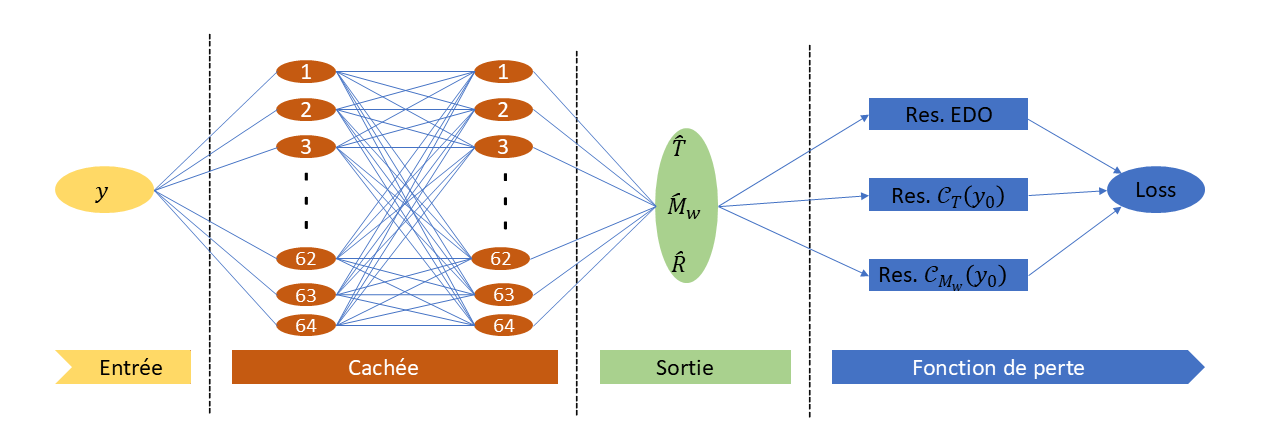
\includegraphics[width=0.7\linewidth]{pp6}
	\captionof{figure}{Structure du réseau}
\end{center}
	\end{frame}
	
	\begin{frame}
			\framesubtitle{\textbf{Méthodologie (suite objectif 2)}}
		\frametitle{\textbf{Transition \& résidus pondérés}}
		\begin{itemize}
		\vspace{0.3cm}
		\item[\maltese] \textbf{Gestion de la transition}.\pause
		\begin{itemize}
			\item[$\divideontimes$] Discontinuité en $T=373\,\mathrm{K}$,
			\item[$\divideontimes$] Fonction de transition $\mathcal{X}(T)$ autour de $373\,\mathrm{K}$ tel que :
			\begin{equation}
				\mathcal{X}(T) = \sigma\left(\lambda\left(T-373\right)\right) \text{ avec } \lambda >> 1
			\end{equation}
		\end{itemize}
		\end{itemize}
		
			\begin{block}{Résidus de l'EDO}\pause
			\begin{itemize}
				\item Pour SP1 : $\mathcal{R}_T(y) = \left(1-\mathcal{X}(T)\right)\cdot\left(\frac{d\hat{T}}{dy} + \frac{Q_1(y, \hat{T})}{\gamma_1 \hat{R}}\right)$.
				\item Pour SP2 : $ \mathcal{R}_{M_w}(y) = \mathcal{X}(T)\cdot\left(\frac{d\hat{M_w}}{dy} - \frac{Q_2(y)}{\gamma_2 \hat{R}}\right)$.
			\end{itemize}\pause
		\end{block} 			
	\end{frame}
	
%	\begin{frame}
%		\frametitle{Gestion de la transition}
%		\begin{itemize}
%			\item[\maltese] Gestion de la transition.\pause
%			\begin{itemize}
%				\item Discontinuité en $T=373\,\mathrm{K}$.
%				\item Fonction de transition $\mathcal{X}(T)$ autour de $373\,\mathrm{K}$ tel que :
%				\begin{equation}
%					\mathcal{X}(T) = \sigma\left(\lambda\left(T-373\right)\right) \text{ avec } \lambda >> 1
%				\end{equation}
%			\end{itemize}
			
%			\item[\maltese] Gestion du paramètre $\hat{R}$.\pause
%			\begin{itemize}
%				\item Régularisation de $ \hat{R}$ sur $\left[R_{\text{min}}, R_{\text{max}}\right]$ : 
%				\begin{equation}
%					\hat{R}(\theta_R) = R_{\text{min}} + (R_{\text{max}} -  R_{\text{min}})\cdot\sigma\left(z(\theta_R)\right)
%				\end{equation}
%			\end{itemize}
%			\pause
%			\item[\maltese]  Optimisation :
%			\begin{itemize}
%				\item Phase 1 : Adam (gradients bruités)
%				\item Phase 2 : L-BFGS (précision)
%			\end{itemize
%		\end{itemize}
%	\end{frame}
	
	
	\begin{frame}
		\framesubtitle{\textbf{Méthodologie (suite objectif 2)}}
		\frametitle{\textbf{Résidus des contraintes \& Loss}}
		
		\begin{block}{Résidus des Conditions initiales}\pause
	
			\begin{itemize}
				\item Pour SP1 : $\mathcal{C}_T(y_0) = \hat{T}(a) - T_{a}$.
				\item Pour SP2 : $\mathcal{C}_{M_w} (y_0) = \hat{M}_w(a) - M_{a}$.
			\end{itemize}\pause
		\end{block}
		\vspace{0.5cm}
		\begin{block}{Fonction de perte global (Loss) \texttwelveudash\text{ }  Pénalisation} \pause 
			\begin{align}
			\mathcal{L}( \theta ) = \mathcal{L}_{\text{EDO}} + \lambda_1 \mathcal{C}_T(y_0) + \lambda_2 \mathcal{C}_{M_w} (y_0)
		\end{align}
		\small\[
		\mathcal{L}(\theta) = {\frac{1}{N}\sum_i \mathcal{R}_T(y_i)^2 + \mathcal{R}_{M_w}(y_i)^2}+ \lambda_1 {(\hat{T}(a)-T_a)^2 + \lambda_2 (\hat{M}_w(a)-M_a)^2}
		\]
		\end{block}
	\end{frame}
	
	
	
	% essai 
	
	
%	\begin{frame}
%		\frametitle{Imposition des conditions}
%		\begin{itemize}
%			\item[\maltese] Imposition par la pénalisation			
%			\begin{align}
%				\mathcal{L}( \theta ) = \mathcal{L}_{\text{EDO}} + \lambda\mathcal{L}_{\text{CI}}
%			\end{align}
%			\small\[
%			\mathcal{L}(\theta) = {\frac{1}{N}\sum_i \mathcal{R}_T(y_i)^2 + \mathcal{R}_{M_w}(y_i)^2}+ \lambda_1 {(\hat{T}(a)-T_a)^2 + \lambda_2 (\hat{M}_w(a)-M_a)^2}
%			\]
%			\pause
%			\item[\maltese]  Imposition par la transformation exacte. 
%			\begin{equation}
%				\mathcal{L}( \theta ) = \mathcal{L}_{\text{EDO}}
%			\end{equation}
%			
%			{ Avec } $\hat{T}(y) = T_{a} + (y-a) \cdot\mathcal{N}_T(y; \theta_T)$  \\
%			\vspace{1ex}
%			et $ \hat{M_w}(y) = M_{a}+ (y-a)\cdot\mathcal{N}_M(y; \theta_M)$
%			%			Où $\mathcal{N}_T \in [0, 1]$ et $\mathcal{N}_M \in [0, 1]$ sont des sorties du réseau entièrement connectés, mais nuls aux bornes. Ce qui permet d'imposer exactement que $T_{a} = T_{a}$ et  $M_w{(a)} = M_{a}$
%		\end{itemize}
%	\end{frame}
	
	%voir 
	\begin{frame}
		\framesubtitle{\textbf{Méthodologie (suite objectif 2)}}
		\frametitle{\textbf{Cas d'Étude : Heading}}
		\begin{itemize}
			\item[\maltese] Valeur initiale :
			\begin{table}[h]
				\scriptsize
				\begin{tabular}{@{}ll@{}}
					\toprule
					\textbf{Paramètre} & \textbf{Valeur} \\
					\midrule
					\rowcolor{blue!5}
					Longueur $y$ & 12 m \\
					\rowcolor{red!5}
					Température d'ignition $T_{a}$ & 303 K \\
					\rowcolor{blue!5}
					Fraction eau $M_w(a)$ & 0.11 \\
					\bottomrule
				\end{tabular}
			\end{table}
			
			\vspace{0.2cm}
%			\item[\maltese] Données d'étude 
%			\begin{itemize}
%				\item Les données du bouleau blanc de \textbf{Koo \textit{et al.,} (2005)}.
%				\item Les données supposées.
%			\end{itemize} 
			\vspace{0.2cm}
			\item[\maltese] Implémentation : 
			\begin{itemize}
					\item[•] Bibliothèque : Pytorch.
					\vspace{0.2cm}
				\item[•] Logiciel : Python.
				
			
			\end{itemize}
		\end{itemize}
	\end{frame}
	
	
	\begin{frame}[plain]
		\noindent
		\includegraphics[width=\paperwidth, height=\paperheight]{pp4.png}
	\end{frame}
	
	\begin{frame}
		\framesubtitle{\textbf{Résultats (objectif 1)}}
		\frametitle{\textbf{Analyse complète du modèle}}
	
		\section{Résultats \& Discussion}
		\pause
		\begin{itemize}
			\item[\maltese] \textbf{Nature du système :} Système hybride d'EDO à transition conditionnelle activée par $T = 373\,\mathrm{K}$ entre SP1/SP2.
			\pause
			\vspace{0.3cm}
			\item[\maltese] \textbf{Existence d'une solution} forte assurée au sens de \textit{Filippov}.
			\pause
			\vspace{0.3cm}
			\item[\maltese] \textbf{Échec de la résolution analytique :} Complexité de $Q_1(y,T)$ et détection impossible des points $y_1$, $y_2$ .
			\pause
			\vspace{0.3cm}
			\item[\maltese] \textbf{Limites des méthodes numériques classiques :}  
			Euler, RK2 et RK3 inadaptées; seule la méthode \textbf{RK4} donne de bon résultat.
		\end{itemize}
		
		%	"Avant de passer à l’implémentation des PINNs, nous avons effectué une analyse complète du modèle.
		%	D'abord, il s'agit d’un système hybride à transition conditionnelle, donc avec des changements de régime selon la température.
		%	Ensuite, la discontinuité à $T = 373,\mathrm{K}$ exclut les théorèmes classiques, mais une solution globale est assurée par l'inclusion de Filippov.
		%	Côté analytique, même en linéarisant les flux, on ne peut pas expliciter les intégrales ou déterminer les points de transition $y_1$ et $y_2$, donc pas de solution fermée.
		%	Enfin, les méthodes numériques standards échouent à cause du saut brutal. Seule la méthode RK4 combinée à une procédure de tir permet de retrouver des résultats cohérents, mais elle ne détermine pas $R$ automatiquement."
	\end{frame}
	
	\begin{frame}
		\frametitle{\textbf{Profils séparés de $T(y)$ et $M_w(y)$}}
		\framesubtitle{\textbf{Résultats (objectif 2)}}
		\begin{itemize}
			\item $T$ croît lentement jusqu'à $373\,\mathrm{K}$, puis plus vite jusqu'à $556.6\,\mathrm{K}$
			\item $M_w$ reste stable puis décroît rapidement après évaporation
		\end{itemize}
		\begin{center}
			\includegraphics[width=0.85\linewidth]{py3}
			\captionof{figure}{Profils séparés de la température $T$ et de l'humidité $M_w$ en fonction de $y$}
		\end{center}
		
		%	Avant de cliquer :
		%	
		%	"Nous allons maintenant examiner les résultats obtenus par les PINNs, en commençant par les profils individuels de la température et de l’humidité en fonction de la distance au front de flamme."
		%	
		%	Une fois affichée :
		%	
		%	"On observe une montée progressive de la température jusqu'à 373 K, puis une accélération liée à l'assèchement du combustible. L'humidité, elle, reste stable au départ, puis chute brusquement une fois ce seuil atteint."
	\end{frame}
	
	
	\begin{frame}
		\frametitle{\textbf{Profils combinés de $T(y)$ et $M_w(y)$}}
		\framesubtitle{\textbf{Résultats (suite objectif 2)}}
		\begin{itemize}
			\item Détection exacte de la transition autour de $373\,\mathrm{K}$.
			\item Apprentissage simultané réussi des deux profils avec {$R = 0.068$} m/s .
		\end{itemize}
		
		
		\begin{center}
			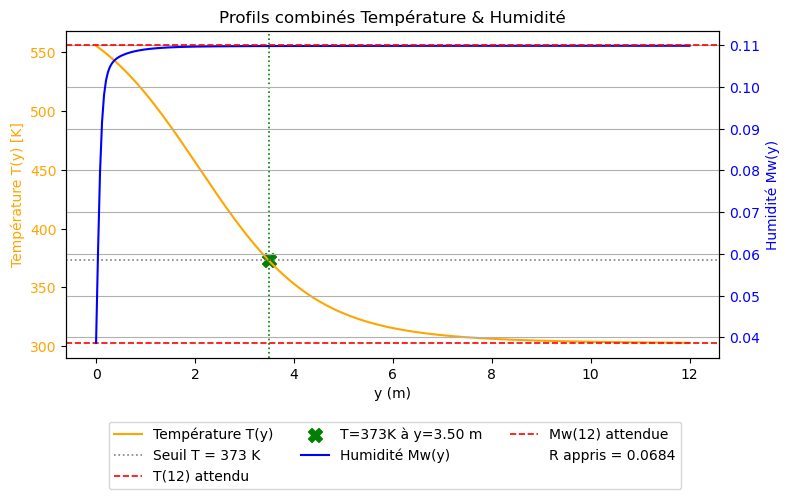
\includegraphics[width=0.75\linewidth]{py6}
			\captionof{figure}{Profils combinés de $T$ et $M_w$ selon la distance $y$}
		\end{center}
	
	\end{frame}
	
	
	\begin{frame}
		\frametitle{\textbf{Contribution des flux thermiques}}
		\framesubtitle{\textbf{Résultats (suite objectif 2)}}
		
	\begin{itemize}
			\item Profils cohérents avec les données physiques et simulation RK4
		\end{itemize}
%		\begin{itemize}
%			\item Flux surfaciques dominants : $q_{\text{rs}}, q_{\text{cs}}$
%			\item Flux internes négligeables : $q_{\text{ri}}, q_{\text{ci}}$
%		\end{itemize}
		
		\begin{center}
			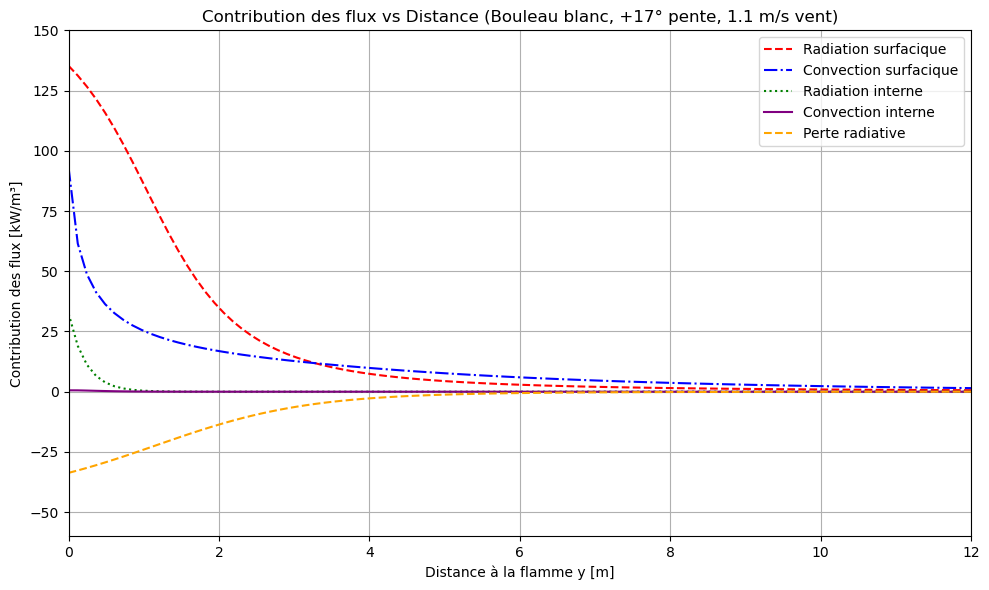
\includegraphics[width=0.75\linewidth]{py5}
			\captionof{figure}{Contributions respectives des flux thermiques en fonction de $y$}
		\end{center}
	
	\end{frame}
	
	
	\begin{frame}
		\frametitle{\textbf{Valeurs numériques des profils et flux}}
		\framesubtitle{\textbf{Résultats (suite objectif 2)}}
		\begin{itemize}
			\item Vitesse apprise : \textcolor{red}{$R = 0.068$} m/s
		\end{itemize}
		
\begin{center}
	\begin{table}[h]
		\footnotesize
		\caption{Valeurs numériques des profils et flux thermiques}
		\begin{tabular}{@{}l*{8}{r}@{}}
			\toprule
			\rowcolor{blue!10}
			$y$ (m) & $T$ (K) & $M_w$ & $q_{rs}$ & $q_{cs}$ & $q_{ri}$ & $q_{ci}$ & $q_{pr}$ & $Q_1$ \\
			\midrule
			\rowcolor{red!5}
			0.0  & 556.6 & 0.039 & 135.2 & 92.8 & 32.3 & 0.7 & -33.7 & 227.4 \\
			\rowcolor{blue!5}
			1.0  & 535.8 & 0.106 & 86.0 & 25.2 & 0.4 & 0.1 & -24.0 & 87.7 \\
			\rowcolor{red!5}
			2.0  & 456.7 & 0.109 & 34.8 & 16.8 & 0.0 & 0.0 & -13.6 & 38.0 \\
			\rowcolor{yellow!15} % Ligne en jaune pâle
			4.0  & 353.1 & 0.110 & 7.4 & 9.9 & 0.0 & 0.0 & -2.8 & 14.5 \\
			\rowcolor{red!5}
			6.0  & 315.5 & 0.110 & 2.9 & 6.0 & 0.0 & 0.0 & -0.6 & 8.3 \\
			\rowcolor{blue!5}
			8.0  & 306.4 & 0.110 & 1.5 & 3.7 & 0.0 & 0.0 & -0.2 & 5.0 \\
			\rowcolor{red!5}
			12.0 & 303.0 & 0.110 & 0.6 & 1.5 & 0.0 & 0.0 & -0.0 & 2.1 \\
			\bottomrule
		\end{tabular}
	\end{table}
\end{center}
		%	Avant de cliquer :
		%	
		%	"Enfin, voici un tableau numérique qui résume l’évolution des différentes grandeurs physiques mesurées tout au long du profil."
		%	
		%	Une fois affichée :
		%	
		%	"On peut y retrouver les valeurs exactes de température, humidité, flux individuels et chaleur totale selon la position. À noter que la vitesse de propagation $R$ apprise automatiquement est d’environ 0.068, proche de celle obtenue par RK4."
	\end{frame}

	\begin{frame}
		\frametitle{\textbf{Conclusion}}
		\section{Conclusion \& Perspectives}
		\begin{itemize}
			\item Analyse (existence de solution, resolution analytique et numérique).
				\vspace{0.3cm}
			\item L'approche par \textbf{PINNs} a permis d'obtenir une solution continue et différentiable tout en apprenant simultanément $T(y)$, $M_w(y)$ et $R$.
		\end{itemize}
	
		
%		Toutefois en dépit de la capacité des PINNs à capturer la dynamique du système, leur coût d'entraînement reste  et les performances restent inférieures aux méthodes classiques pour les problèmes directs. \\
		\pause
		\vspace{0.4cm}
		Cette étude valide l'application des PINNs aux systèmes hybrides, sous réserve d'une bonne gestion des discontinuités.
		
	\end{frame}
	
	\begin{frame}
		\frametitle{\textbf{Perspectives}}
%		Pour égaler la précision des méthodes numériques comme RK4 et les résultats obtenus par \textbf{Koo \textit{et al}., (2005)} : %il s'avère important de proposer les perspectives suivantes : 
		
		\begin{itemize}
			\item[$\maltese$] \textbf{Méthode de tir + PINNs} pour respecter exactement les conditions de référence. 
			\pause
			\vspace{0.4cm}
			\item[$ \maltese$]	\textbf{Méthode  numériques classiques} permet de capturer la transition, avant d'appliquer les \textbf{PINNs} sur chaque régime individuellement. \pause
			\vspace{0.4cm}
			\item[$\maltese$] \textbf{XPINNs (Extended PINNs)} : adapter aux transitions brutales et permet d'améliorer la stabilité de l'entraînement.
		\end{itemize}
	\end{frame}
	
%	\begin{frame}
%		\frametitle{Remerciements }
%		
%		% Police élégante (choisir selon ce qui est disponible)
%		\fontfamily{phv}\selectfont % Helvetica
%		% Alternatives: \usepackage{mathpazo} pour Palatino, ou \usepackage{arev} etc.
%		
%		\centering
%		\vspace{1cm}
%		\textcolor{blue!85!black}{\textbf{\Huge MERCI À TOUS}}\\
%		\vspace{0.5cm}
%		\textcolor{blue!75!black}{\textbf{\Huge POUR VOTRE}}\\
%		\vspace{0.5cm}
%		\textcolor{blue!65!black}{\textbf{\Huge AIMABLE ATTENTION !}}
%	\end{frame}
	
%	\begin{frame}{}
%		\centering
%		\textcolor{blue!85!black}{\textbf{\Huge MERCI À TOUS}}\\
%	\vspace{0.2cm}
%	\textcolor{blue!75!black}{\textbf{\huge POUR VOTRE}}\\
%	\vspace{0.2cm}
%	\textcolor{blue!65!black}{\textbf{\Large AIMABLE ATTENTION !}} \\
%		\vspace{0.2cm}
%		\includegraphics[width=0.3\textwidth]{upgc2-removebg-preview.png} \\
%	%	\footnotesize dalano2910@gmail.com \\ 
%%	\footnotesize La toute première soutenance de master de Mathématique l'histoire de l'UPGC.
%		\footnotesize Soutenance : \today \\
%	\vspace{0.1cm}
%	%	\footnotesize Comme un aigle, je m'élève au-dessus de chaque obstacle.
%	\footnotesize Encadreur : \hfil Président :  \hfil Examinateur : \\
%	\footnotesize Dr N'Gohisse K.Firmin \hfil Dr Coulibaly Kouame \hfil Dr N'ZI Y.Guillaume
%	\end{frame}
	
	\begin{frame}[plain]
		\noindent
		\includegraphics[width=\paperwidth, height=\paperheight]{pp5.png}
	\end{frame}	
	
	%===========================================================
	
\end{document}